% THIS TEMPLATE IS A WORK IN PROGRESS

\documentclass{article}
\usepackage{graphicx}
\usepackage{hyperref}
\usepackage{fancyhdr}
\usepackage{float}
\usepackage{hyperref}

% FOR CODE
\usepackage{listings}
\usepackage{xcolor}
\usepackage{xparse}
\NewDocumentCommand{\codeword}{v}{%
\texttt{{#1}}%
}

\definecolor{codegreen}{rgb}{0,0.6,0}
\definecolor{codegray}{rgb}{0.5,0.5,0.5}
\definecolor{codepurple}{rgb}{0.58,0,0.82}
\definecolor{backcolour}{rgb}{0.95,0.95,0.92}

\lstdefinestyle{mystyle}{
    backgroundcolor=\color{backcolour},   
    commentstyle=\color{codegreen},
    keywordstyle=\color{magenta},
    numberstyle=\tiny\color{codegray},
    stringstyle=\color{codepurple},
    basicstyle=\ttfamily\footnotesize,
    breakatwhitespace=false,         
    breaklines=true,                 
    captionpos=b,                    
    keepspaces=true,                 
    numbers=left,                    
    numbersep=5pt,                  
    showspaces=false,                
    showstringspaces=false,
    showtabs=false,                  
    tabsize=2
}

\lstset{style=mystyle}
% 

\fancypagestyle{firstpage}{%
  \lhead{CAP6610 Project Progress Report}
  \rhead{Akash Gajjar}
}

\begin{document}
\thispagestyle{firstpage}

\section{Summary}
Since I was able to successfully load the dataset and explore the dataset I have started implementing the GAN. I have looked at the GAN paper and figured out some details that might help me in implementing the GAN. I am using \codeword{pytorch} library to implement the generator and discriminator but faced some issue in setting up the models. Mainly the issues are with shape mismatch in vector related operations. The \codeword{pytorch} documentation has been really helpful in fixing the mistakes based on the type of inputs that the functions accept. I am taking a reference from \codeword{DCGAN} implementation from pytorch examples repository\cite{1}. One thing that I am planning to do after loading the data is to normalize the input data (understood normalization through the lecture). 

\section{Model Architecture}

\subsection{Generator}
The generator architecture is inspired from the architecture given in the \codeword{DCGAN}\cite{2} paper.
\begin{figure}[H]
  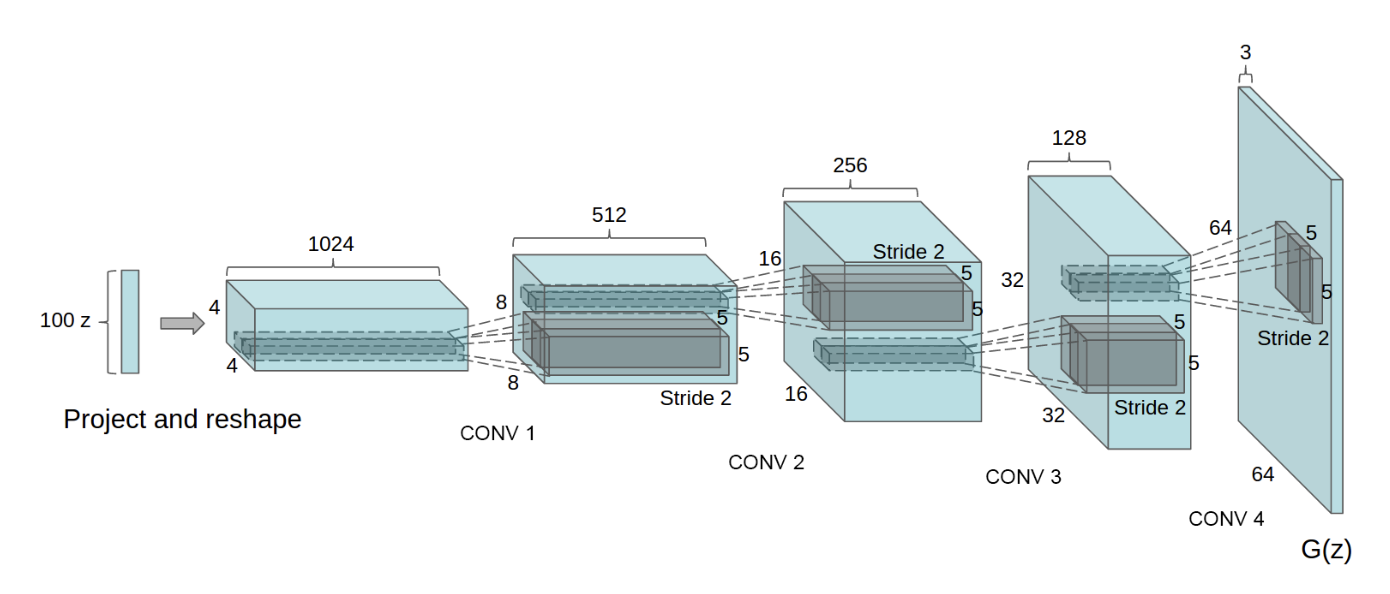
\includegraphics[width=\linewidth]{images/architecture.png}
\end{figure}
This is how it's set up using \codeword{pytorch}, number of channels in various hidden layers is different than given in the above architecture. I am inputting 100 latent features to the generator and it generates a $64\times64$ single channel (greyscale) image.
\begin{lstlisting}[language=Python]
nn.Sequential(
    # input is Z, going into a convolution
    nn.ConvTranspose2d(     nz, ngf * 8, 4, 1, 0, bias=False),
    nn.BatchNorm2d(ngf * 8),
    nn.ReLU(True),
    # state size. (ngf*8) x 4 x 4
    nn.ConvTranspose2d(ngf * 8, ngf * 4, 4, 2, 1, bias=False),
    nn.BatchNorm2d(ngf * 4),
    nn.ReLU(True),
    # state size. (ngf*4) x 8 x 8
    nn.ConvTranspose2d(ngf * 4, ngf * 2, 4, 2, 1, bias=False),
    nn.BatchNorm2d(ngf * 2),
    nn.ReLU(True),
    # state size. (ngf*2) x 16 x 16
    nn.ConvTranspose2d(ngf * 2,     ngf, 4, 2, 1, bias=False),
    nn.BatchNorm2d(ngf),
    nn.ReLU(True),
    # state size. (ngf) x 32 x 32
    nn.ConvTranspose2d(    ngf,      nc, 4, 2, 1, bias=False),
    nn.Tanh()
    # state size. (nc) x 64 x 64
)
\end{lstlisting}

\subsection{Discriminator}

Discriminator has a kind of similar architecture as generator but reversed. It takes a single channel $64 \times 64$ image and outputs a single value through a sigmoid function.

\section{Next Steps}

Now that I have set up the higher level details of the model, I need to set up the forward propagation as well as decide on the optimizer to use and how I am going to do the back propagation and perform training of the network. I also have to decide various hyper-parameters of the model and see which values yield the best results. Hopefully I will be able to generate some images after I setup the initial training.

\begin{thebibliography}{1}

\bibitem{1} \url{https://github.com/pytorch/examples/tree/main/dcgan}
\bibitem{2} \url{https://arxiv.org/pdf/1511.06434.pdf}
\end{thebibliography}

\end{document}
